\begin{figure}[htbp]
  \begin{tabular}{ccc}
    \begin{minipage}{0.33\hsize}
      \centering
      \dKNpimSp\\
      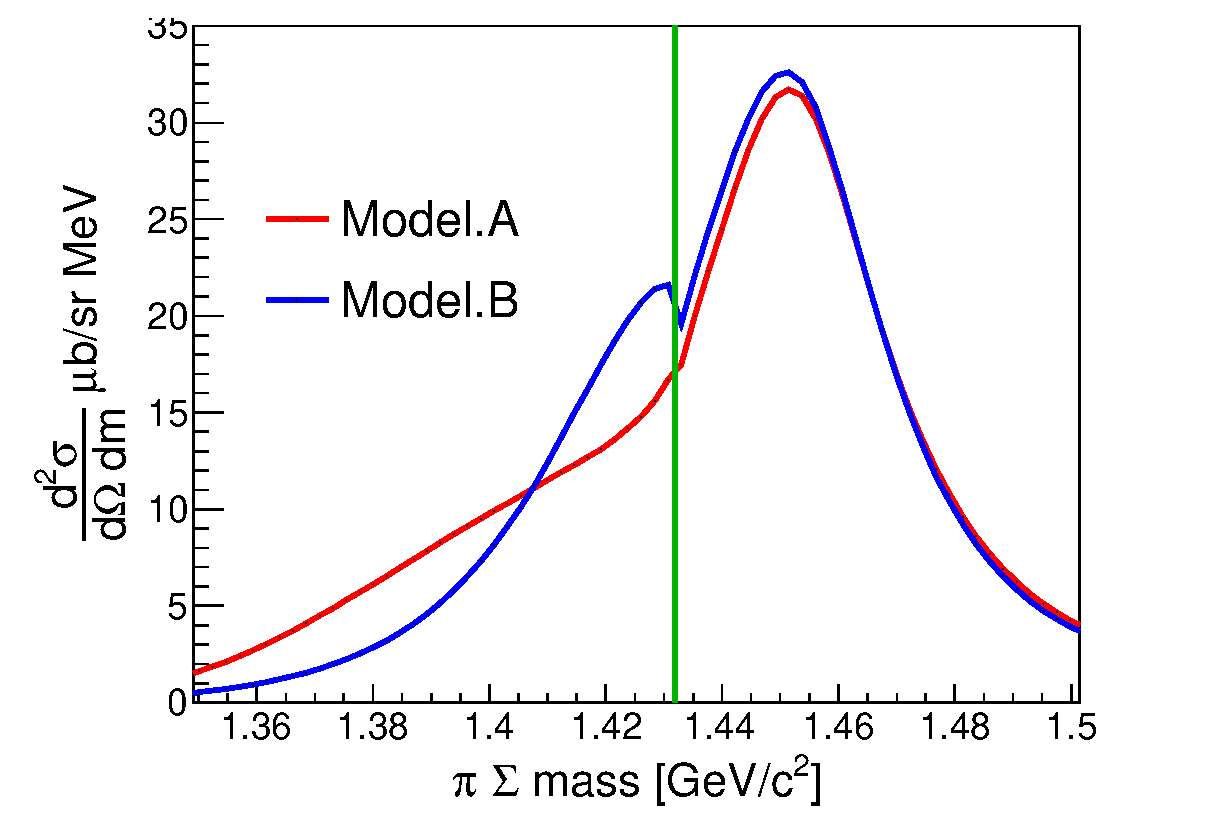
\includegraphics[width=4.3cm]{../pic/discussion/DCC_pimSp.eps}
    \end{minipage}

    \begin{minipage}{0.33\hsize}
      \centering
      \dKNpipSm\\
      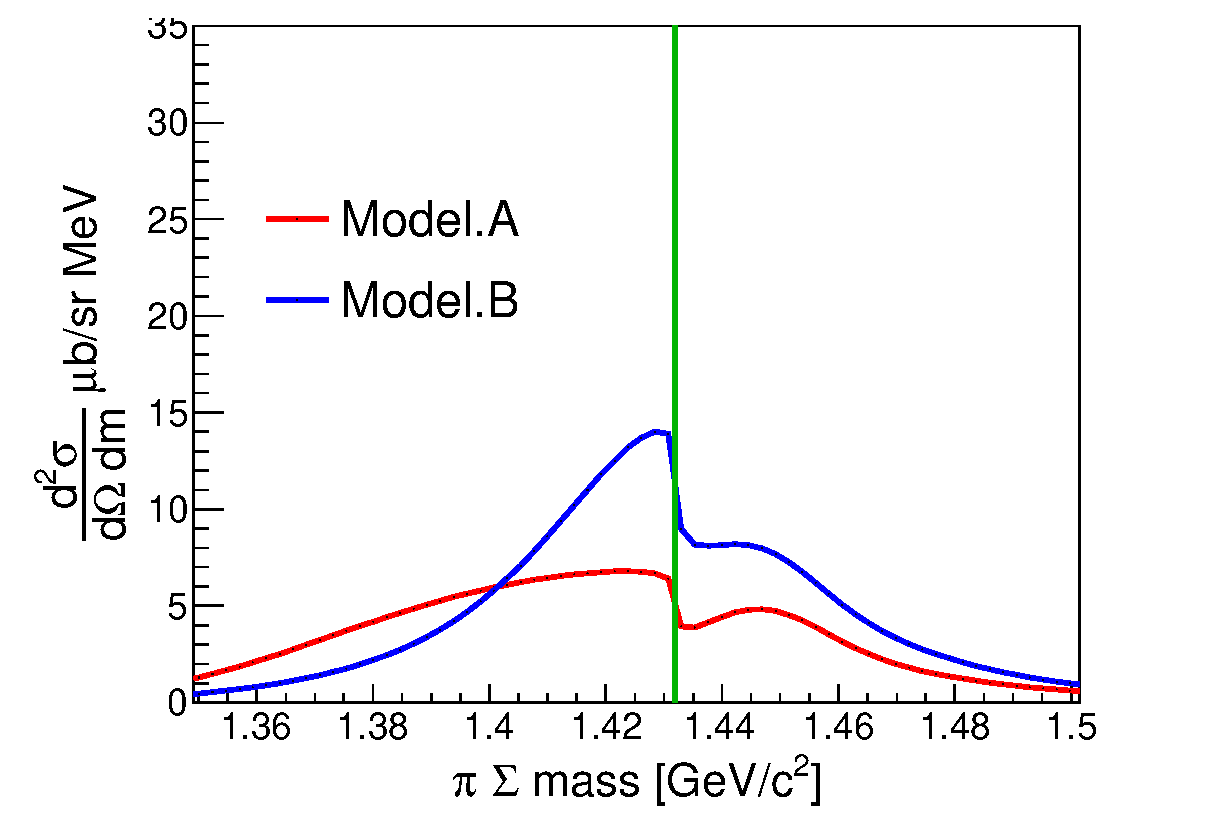
\includegraphics[width=4.3cm]{../pic/discussion/DCC_pipSm.eps}
    \end{minipage}

    \begin{minipage}{0.33\hsize}
      \centering
      \dKPpimSz\\
      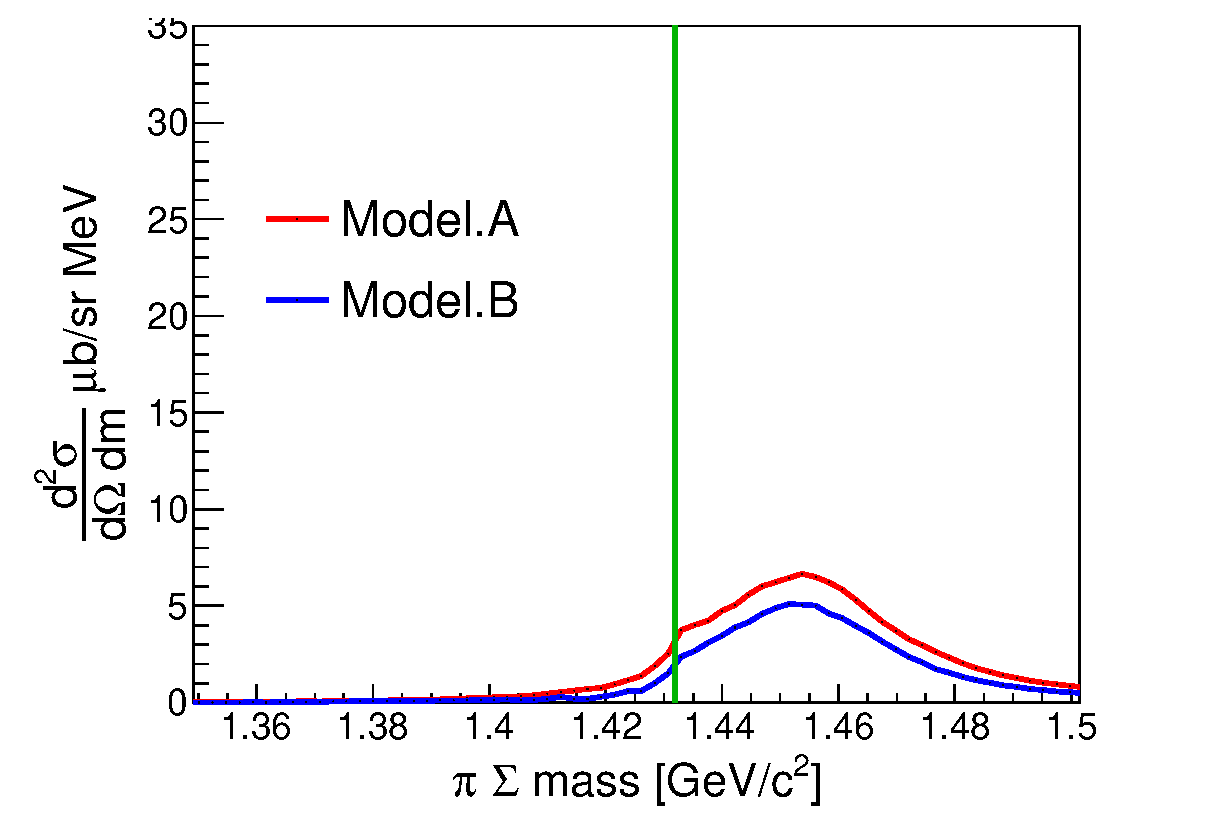
\includegraphics[width=4.3cm]{../pic/discussion/DCC_pimS0.eps}
    \end{minipage}
  \end{tabular}
  \caption{
    The calculated spectra by the DCC method \cite{DCC2}.
    Left, center and right figures show \pimSp, \pipSm and \pimSz, respectively.
    Red and blue lines represent model.A and B, respectively.
    Green vertical line indicates the $K^-p$ mass threshold.
  }
  \label{fig:DCC_kd}
\end{figure}
